\documentclass[11pt,a4paper]{article}

\usepackage[margin=2.5cm]{geometry}
\usepackage[T1]{fontenc}
\usepackage{lmodern}
\usepackage{graphicx}
\usepackage{booktabs}
\usepackage{array}
\usepackage{float}
\usepackage[hidelinks]{hyperref}

% Figures are produced by `python -m src.eval.figures` (TICK-403).
\graphicspath{{../artifacts/tick-403/}{artifacts/tick-403/}{figures/}}

\newcolumntype{L}[1]{>{\raggedright\arraybackslash}p{#1}}
\newcolumntype{R}[1]{>{\raggedleft\arraybackslash}p{#1}}

\title{Project Ascent: Building a Small Language Model from Scratch\\
\large Tokenizers, Adaptation, Retrieval, Prompting and a Tool-Using Agent}
\author{Project Ascent}
\date{October 2026}

\begin{document}
\maketitle

\begin{abstract}
Project Ascent builds a decoder-only Transformer language model end to end on a CPU-sized budget and
extends it in four phases: a character-level baseline, a trained BPE tokenizer with architectural
variants, LoRA fine-tuning plus lexical retrieval, and a prompt-chain agent with memory and a safe
calculator. This report records what was built and what was measured. All trained models are tiny
(about $1.1\times10^{5}$ parameters, 500 optimisation steps, TinyShakespeare, one seed). The only
head-to-head comparison with real numbers is character versus BPE tokenization, where BPE reaches
3.09 versus 3.45 validation bits per character. Prompting, instruction-following and agent
experiments verify the \emph{pipelines}; they do not show useful model capability, and no such
claim is made.
\end{abstract}

\section{System overview}

\begin{table}[H]
\centering
\begin{tabular}{L{3.2cm}L{11.3cm}}
\toprule
Component & Implementation \\
\midrule
Model & Decoder-only \texttt{MiniGPT}: learned positions, tied embeddings, causal self-attention,
        LayerNorm or RMSNorm, PyTorch scaled-dot-product attention with a manual fallback \\
Tokenizers & Deterministic character tokenizer (\texttt{<unk>} = ID 0); deterministic
             character-initialised BPE with JSON-serialised merges \\
Decoding & Greedy, beam, top-$k$ and top-$p$ \\
Training & Argparse plus optional YAML, CPU/CUDA selection, checkpoints with optimizer state and
           resume compatibility checks \\
Adaptation & Alpaca-style formatting with prompt-loss masking; frozen-base LoRA on the attention
             \texttt{qkv} and output projections \\
Retrieval & Dependency-free lexical chunk retrieval with source provenance and bounded prompts \\
Agent & Memory window, \texttt{/calc} command, model-requested \texttt{CALC(...)} calls, bounded
        tool rounds, AST-based calculator (no \texttt{eval}) \\
\bottomrule
\end{tabular}
\caption{Implemented architecture. Every ticket has automated tests; the suite is run with
\texttt{python -m unittest discover -s tests}.}
\end{table}

\section{Phase 1 and 3 smoke runs}

These runs show that the plumbing works. They are not quality evidence.

\begin{table}[H]
\centering
\begin{tabular}{L{3.6cm}L{6.2cm}L{4.7cm}}
\toprule
Run & Configuration & Result \\
\midrule
Baseline smoke & 1 layer, 32 dim, 4 heads, 32 context, 8 steps &
  Validation loss 4.1424 $\to$ 3.9212; perplexity 62.96 $\to$ 50.46 \\
LoRA smoke & 3 instructions, rank 2, 6 steps &
  384 trainable parameters; final supervised loss 4.0325 \\
RAG smoke & Query ``Which planet is red?'' &
  Retrieved \texttt{knowledge.txt}, lexical score 0.75; generated text was not an answer \\
\bottomrule
\end{tabular}
\caption{Smoke-test results. The undertrained baseline produced degenerate text; retrieval and
provenance work, while answer quality would need a substantive training run.}
\end{table}

\section{Character versus BPE tokenization}

\paragraph{Setup.} Both models use TinyShakespeare, seed 42, 2 layers, 64 dimensions, 4 heads, context
64, batch size 16, learning rate $10^{-3}$, 500 steps, CPU. BPE uses 100 merges.

\begin{table}[H]
\centering
\begin{tabular}{L{6.4cm}R{3.4cm}R{3.4cm}}
\toprule
Metric & Character & BPE \\
\midrule
Vocabulary size & 66 & 166 \\
Parameters & 108,416 & 114,816 \\
Characters per token (validation) & 1.000 & 1.620 \\
Validation loss (per token) & 2.3931 & 3.4757 \\
Perplexity per token (not comparable) & 10.95 & 32.32 \\
Validation bits per character & 3.4525 & 3.0946 \\
Perplexity per character & 10.95 & 8.54 \\
Greedy repetition (char 3-gram) & 0.970 & 0.742 \\
Sampled repetition (char 3-gram) & 0.126 & 0.091 \\
Greedy / sampled characters per second & 3429 / 3144 & 4148 / 4277 \\
\bottomrule
\end{tabular}
\caption{Character versus BPE (single seed). Per-token perplexity is shown only to explain why it must
not be compared: a BPE token carries 1.62 characters on average.}
\end{table}

\begin{figure}[H]
\centering
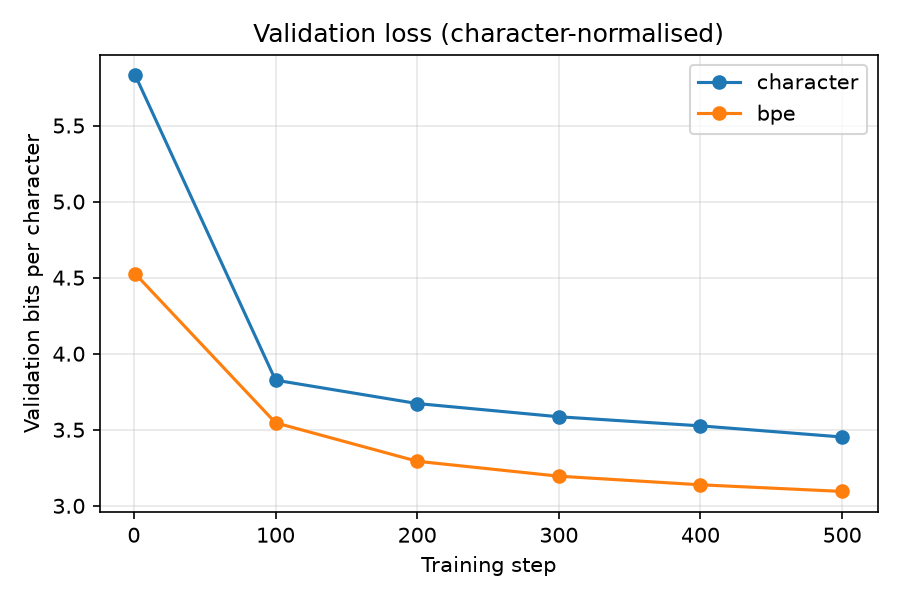
\includegraphics[width=0.78\linewidth]{loss_curves.png}
\caption{Validation loss converted to bits per character using each run's measured
characters-per-token ratio. BPE is lower at every evaluated step.}
\end{figure}

\begin{figure}[H]
\centering
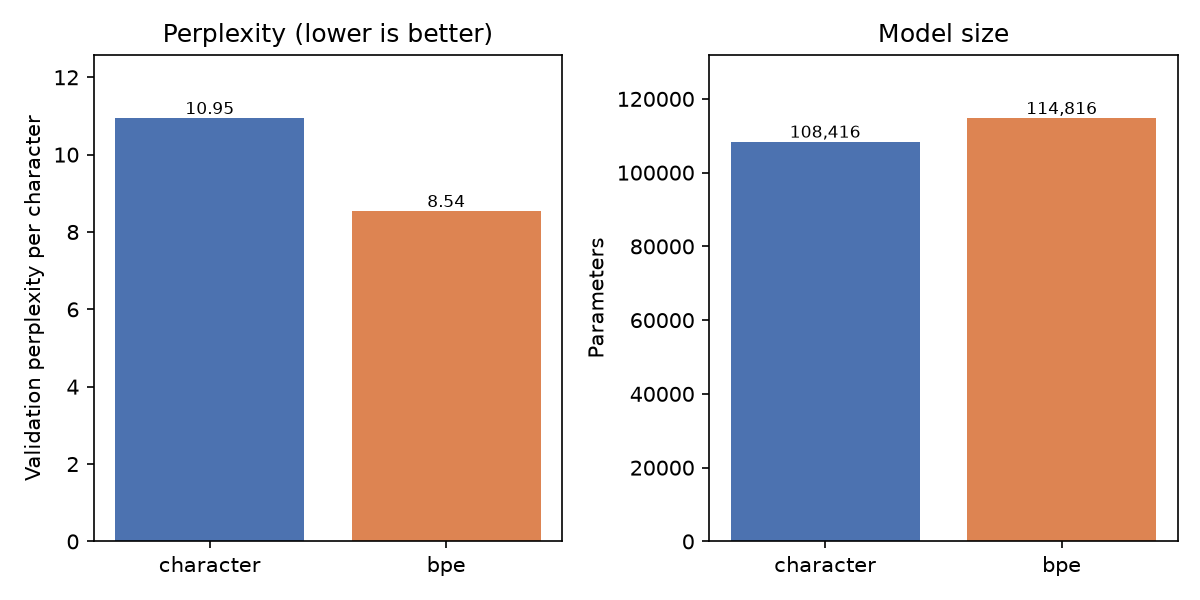
\includegraphics[width=\linewidth]{perplexity_params.png}
\caption{Per-character perplexity and parameter counts. BPE costs 6,400 extra parameters (5.9\%), all
from the 100 additional embedding rows.}
\end{figure}

\begin{figure}[H]
\centering
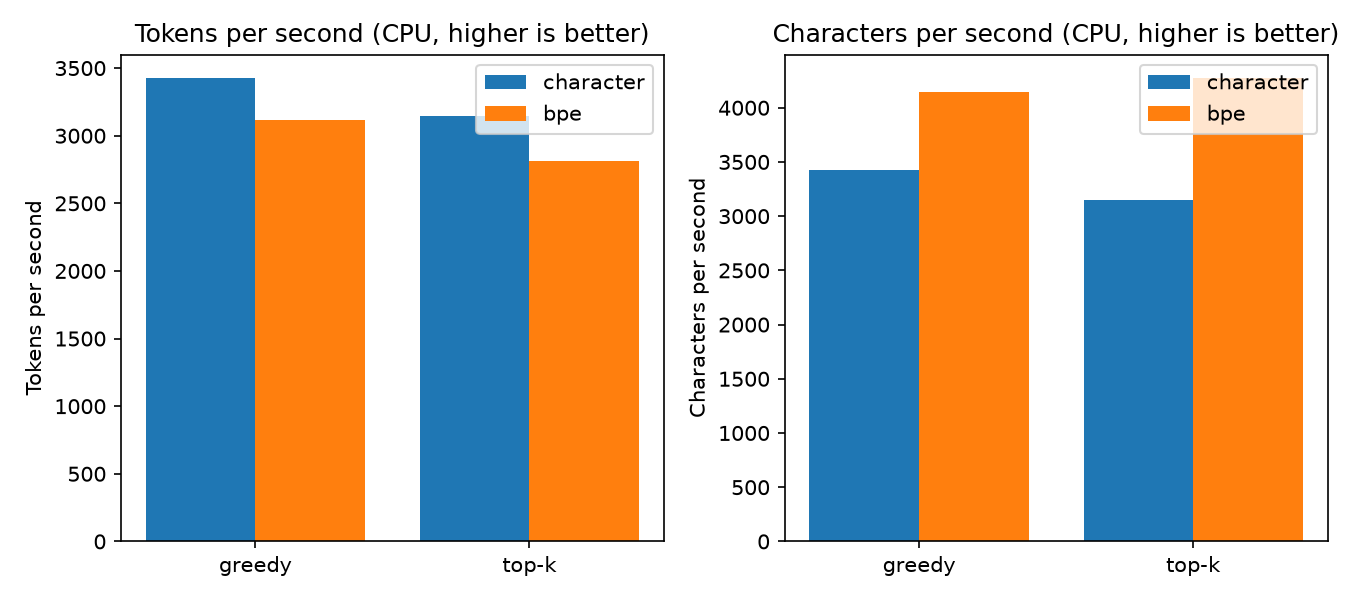
\includegraphics[width=\linewidth]{latency.png}
\caption{Generation speed on CPU from one 200-token sample per mode. BPE is slower per token but
produces more characters per second because each step emits more than one character.}
\end{figure}

\paragraph{Interpretation.} On the character-normalised scale BPE is about 10\% better in bits per
character and repeats less. Greedy output loops in both models. BPE samples contain more real words,
but both models are heavily undertrained, so this is a relative signal only.

\paragraph{Confounds.} (i) With a fixed 64-token context, BPE sees roughly 104 characters per window and
about 1.6$\times$ more text per step, so part of its advantage may come from data exposure rather than
tokenization quality. (ii) BPE merges were learned on the full corpus, including validation text.
(iii) Validation loss uses 20 random batches, not a full sweep. (iv) One seed and one merge count give
no variance estimate. (v) The 28.2 s versus 5.0 s wall-clock figure includes pure-Python BPE training
and encoding and is not a training-throughput comparison.

\section{Attention inspection}

\begin{figure}[H]
\centering
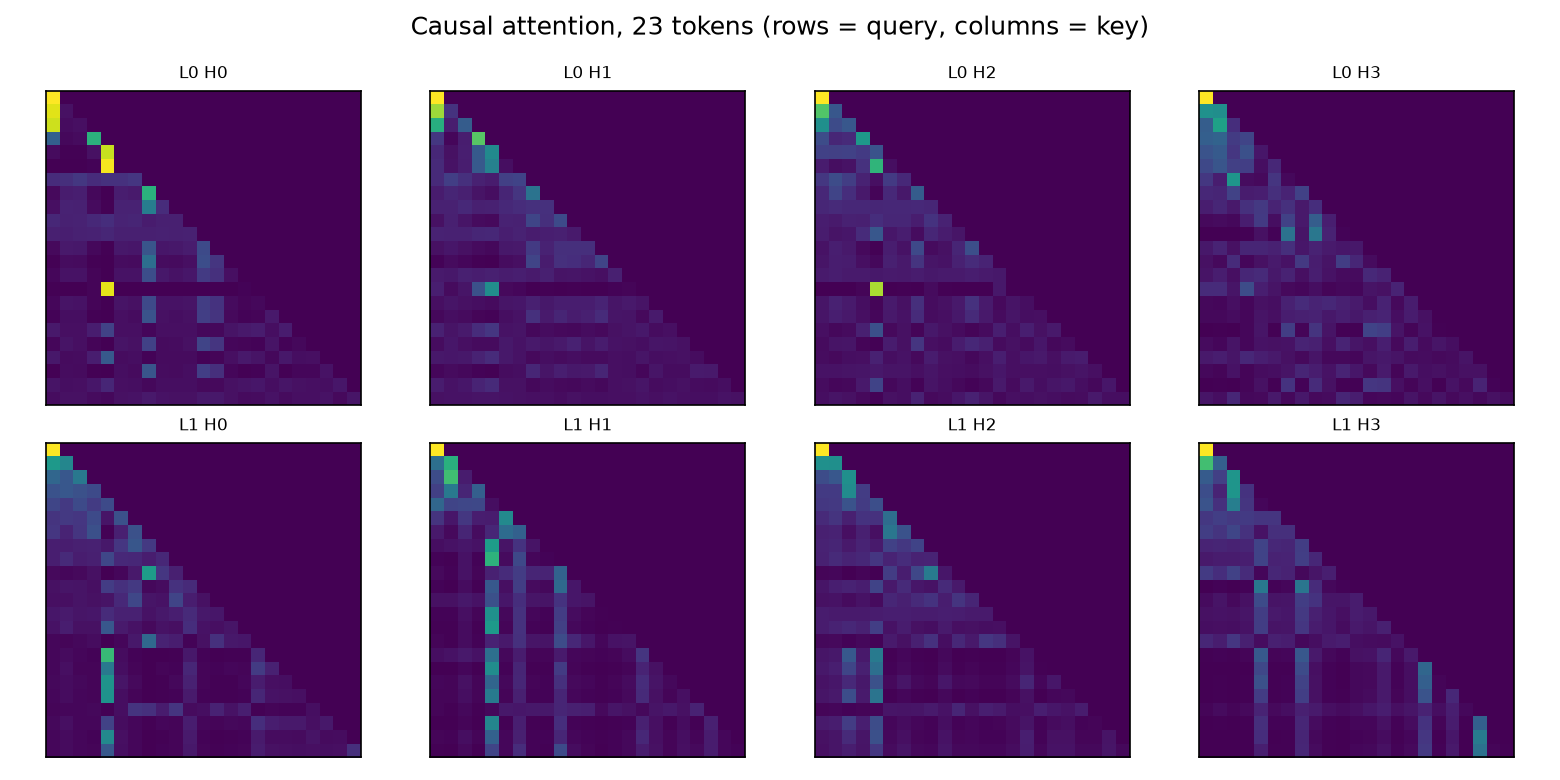
\includegraphics[width=\linewidth]{attention.png}
\caption{Per-head causal attention maps for the BPE model on a 23-token prompt (rows are queries,
columns are keys). Every map is lower-triangular, as required by causal masking. Some heads show
strong attention to the first token and a few vertical stripes. With 500 training steps this
illustrates the extraction tooling; it is not evidence of learned linguistic structure.}
\end{figure}

\section{Prompting}

Zero-shot, few-shot (2 shots) and chain-of-thought prompts were run greedily on six arithmetic and
factual tasks, with numbers spelled out because the corpus has almost no digits.

\begin{table}[H]
\centering
\begin{tabular}{L{3.0cm}L{2.6cm}R{2.4cm}R{3.0cm}R{2.8cm}}
\toprule
Checkpoint & Style & Exact / contains & Prompt truncated & Mean prompt tokens \\
\midrule
BPE & zero-shot & 0/6 & 0\% & 25.3 \\
BPE & few-shot & 0/6 & 100\% & 72.3 \\
BPE & CoT & 0/6 & 100\% & 174.3 \\
Character & zero-shot & 0/6 & 0\% & 37.5 \\
Character & few-shot & 0/6 & 100\% & 104.5 \\
Character & CoT & 0/6 & 100\% & 263.5 \\
\bottomrule
\end{tabular}
\caption{Prompting results. All styles score zero, so no ranking of prompt styles is claimed.}
\end{table}

The measurable effect is context budget: with a 64-token window every few-shot and CoT prompt is
cropped, which removes the exemplars. BPE needs about 0.67$\times$ the prompt tokens of the character
model for the same text, a practical benefit for in-context prompting.

\section{Agent: memory and calculator}

The agent builds each prompt from a preamble and the newest conversation turns that fit a character
budget, then optionally executes a calculator call and feeds the result back, for at most two rounds.
The calculator parses with \texttt{ast} and whitelists numeric literals, \texttt{+ - * / // \% **} and
unary signs. It limits expressions to 200 characters, nesting to depth 50, exponents to magnitude 100
and results to $10^{100}$.

\begin{table}[H]
\centering
\begin{tabular}{L{4.6cm}L{9.9cm}}
\toprule
Input & Observed result \\
\midrule
\texttt{/calc (2+3)*4} & \texttt{20} (no model call) \\
\texttt{/calc 2**1000} & Rejected: exponent magnitude is limited to 100 \\
\texttt{/calc \_\_import\_\_('os')} & Rejected: unsupported syntax (call) \\
Second process, same memory file & 10 turns loaded (8 saved plus 2 new) \\
\bottomrule
\end{tabular}
\caption{Owner-run demo on the BPE checkpoint; 42 tests passed at that point.}
\end{table}

\paragraph{Limitations.} The 500-step models cannot emit \texttt{CALC(...)} themselves, so
model-initiated tool use is verified only with scripted stubs; the working tool path is \texttt{/calc}.
Digits are \texttt{<unk>} for the character model. Memory is a recency window, not summarisation or
retrieval.

\section{Limitations and conclusion}

\begin{itemize}
\item All trained results are single-seed, 500-step runs of roughly 110k-parameter models on one small corpus.
\item Instruction following and RAG answer quality were not evaluated beyond smoke runs; the retrieval
      and adaptation code paths are tested but their quality is unmeasured.
\item Latency comes from single CPU samples and is indicative only.
\item BPE is course-scale, not production byte-level BPE, and retrieval is lexical only.
\end{itemize}

The supported conclusions are narrow. The full pipeline works and is tested. BPE gives a roughly 10\%
lower bits-per-character than the character baseline in this setup, with the confounds listed above. The
tool layer rejects unsafe expressions and persists memory. Stronger claims would need longer training, a
larger context, multiple seeds and held-out instruction and RAG evaluations.

\end{document}
